\documentclass[a4paper]{oblivoir}
\usepackage{amsmath,amssymb,kotex,mdframed,paralist,tabu}
\usepackage{fapapersize}
\usefapapersize{210mm,297mm,20mm,*,20mm,*}

\usepackage{tabto,pifont}
\TabPositions{0.2\textwidth,0.4\textwidth,0.6\textwidth,0.8\textwidth}

%%% 객관식 선지
\newcommand\one{\ding{172}}
\newcommand\two{\ding{173}}
\newcommand\three{\ding{174}}
\newcommand\four{\ding{175}}
\newcommand\five{\ding{176}}
\usepackage{tabto,pifont}
%\TabPositions{0.2\textwidth,0.4\textwidth,0.6\textwidth,0.8\textwidth}

\newcommand\taba[5]{\par\noindent
\one\:{#1}
\tabto{0.2\textwidth}\two\:\:{#2}
\tabto{0.4\textwidth}\three\:\:{#3}
\tabto{0.6\textwidth}\four\:\:{#4}
\tabto{0.8\textwidth}\five\:\:{#5}}

\newcommand\tabb[5]{\par\noindent
\one\:{#1}
\tabto{0.33\textwidth}\two\:\:{#2}
\tabto{0.67\textwidth}\three\:\:{#3}\medskip\par\noindent
\four\:\:{#4}
\tabto{0.33\textwidth}\five\:\:{#5}}

\newcommand\tabc[5]{\par\noindent
\one\:{#1}
\tabto{0.5\textwidth}\two\:\:{#2}\medskip\par\noindent
\three\:\:{#3}
\tabto{0.5\textwidth}\four\:\:{#4}\medskip\par\noindent
\five\:\:{#5}}

\newcommand\tabd[5]{\par\noindent
\one\:{#1}\medskip\par\noindent
\two\:\:{#2}\medskip\par\noindent
\three\:\:{#3}\medskip\par\noindent
\four\:\:{#4}\medskip\par\noindent
\five\:\:{#5}}

\newcommand\vs[1]{\par\vspace{30pt}}

\usepackage{graphicx}

%\pagestyle{empty}

%%% Counters
\newcounter{num}

%%% Commands
\newcommand{\prob}[1]
{\bigskip\bigskip\noindent\refstepcounter{num}\textbf{문제 \arabic{num})} #1\par\noindent}

\newcommand\pb[1]{\ensuremath{\fbox{\phantom{#1}}}}

\newcommand\ba{\ensuremath{\:|\:}}

\newcommand\an[1]{\bigskip\par\noindent\textbf{문제 #1)}\par\noindent}

%%% Meta Commands
\let\oldsection\section
\renewcommand\section{\clearpage\oldsection}

\let\emph\textsf

\begin{document}
\begin{center}
\LARGE태희, 미니테스트 06
\end{center}
\begin{flushright}
날짜 : 2018년 \(\pb3\)월 \(\pb{10}\)일 \(\pb{월}\)요일
,\qquad
제한시간 : \pb{17년}분
,\qquad
점수 : \pb{20} / \pb{20}
\end{flushright}

%
\prob{실수 \(x\), \(y\)가 \(\displaystyle \frac1x+\frac1{2y}=1\)을 만족시킬 때, \(5^x=9^y=k\)가 성립한다.
상수 \(k\)의 값은?}
\taba
5{15}{25}{35}{45}
\vs

%
\prob{\(9^a+9^{-a}=7\)일 때, \(\displaystyle\frac{3^{6a}+1}{3^{4a}+3^{2a}}\)의 값을 구하시오.}
\vs

%
\prob{어느 세라믹 재료의 열전도 계수(\(\kappa\))는 적절한 실험 조건에서 일정하고, 다음과 같이 계산된다고 한다.}
\[\kappa=C\frac{\log t_2-\log t_1}{T_2-T_1}\]
이때, \(C\)는 0보다 큰 상수이고 \(T_1\)\textdegree{}C. \(T_2\)\textdegree{}C
는 실험을 시작한 후 각각 \(t_1\)초, \(t_2\)초일 때 세라믹 재료의 측정 온도이다.
이 세라믹 재료의 열전도 계수를 측정하는 실험에서 실험을 시작한 후 15초일 때와 30초일 때의 측정 온도가 각각 400\textdegree{}C, 404\textdegree{}C이었다.
측정온도가 412\textdegree{}C가 될 때는 실험을 시작한 지 몇 초 후인지 구하시오.
\vs

%
\prob{함수 \(y=3^{x-a}+b\)의 그래프가 아래 그림과 같을 때, \(a+b\)의 값은?}
(단 \(a\), \(b\)는 상수이고 직선 \(y=-1\)은 점근선이다.)
\begin{center}
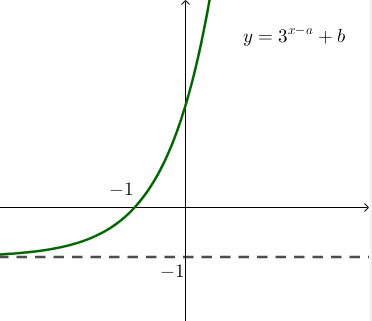
\includegraphics[width=.3\textwidth]{log_function_problem}
\end{center}
\taba{$-2$}{$-1$}012
\vs

%
\prob{다음 함수들의 최댓값과 최솟값을 조사하여라.}
\begin{enumerate}[(1)]
\item
\(y=2^x-2^{\frac12x+2}+6\quad(0\le x\le4)\)
\item
\(y=(\log x)^2+2\log x+6\quad(\frac1{1000}\le x\le1)\)
\item
\(y=\left(\frac12\right)^{x^2-6x+8}\quad(2\le x\le 5)\)
\end{enumerate}

\newpage
%
\prob{수지, 송이, 민준은 각각 서울, 부산, 광주 중에서 서로 다른 도시에 살고 있다.
세 사람은 다음과 같이 말하였다.}
\begin{mdframed}
수지 : 나는 서울에서 살고 있다.\\
송이 : 나는 서울에서 살고 있지 않다.\\
민준 : 나는 광주에서 살고 있지 않다.
\end{mdframed}
세 사람 중에서 한 사람만 진실을 말하였다고 할 때, 서울, 부산, 광주에 살고 있는 사람을 차례로 나열하면?
\par\bigskip\noindent
\begin{tabu}to.4\textwidth{X[0.5]XXX}
		&서울&부산&광주\\
\one		&수지&민준&송이\\
\two		&송이&민준&수지\\
\three	&송이&수지&민준\\
\four		&수지&송이&민준\\
\five		&민준&수지&송이
\end{tabu}
\vs

%
\prob{\(a>0\), \(b>0\)일 때, \(\displaystyle (3a+2b)\left(\frac3a+\frac2b\right)\)의 최솟값은?}
\taba{22}{23}{24}{25}{26}
\vs

%
\prob{\(x>5\)일 때, \(\displaystyle x+\frac1{x-5}\)의 최솟값을 \(m\), 그때의 \(x\)의 값을 \(n\)이라고 할 때, 상수 \(m\), \(n\)에 대하여 \(m+n\)의 값은?}
\taba67{13}{20}{23}
\vs

%
\prob{실수 \(x\), \(y\)에 대하여 \(x^2+y^2=5\)일 때, \(x+2y\)의 최댓값은 \(M\)이고 최솟값은 \(m\)이다.
\(M-m\)의 값은?}
\taba{10}{15}{25}{35}{45}
\vs

%
\prob{모든 실수 \(x\)에 대하여 부등식}
\[k\{x^2+2(k-1)x-5(k-1)\}<0\]
이 성립하도록 하는 정수 \(k\)의 값의 합을 구하여라.
\end{document}